Lab 1

"""

\documentclass{article}
\usepackage{fancyhdr}
\usepackage{lipsum} % for dummy text
\pagestyle{fancy}
\fancyhf{} % Clear header and footer
\fancyhead[R]{Latex Programming} % Right header
\fancyfoot[R]{\thepage} % Right header
\fancyfoot[L]{VVIET, Mysore} % Left footer
\begin{document}
\section{Section 1}
\lipsum[1-2]
\section{Section 2}
\lipsum[1]
\end{document}

"""

Lab 2

"""

\documentclass {article} 
\usepackage{lipsum}
\usepackage {fancyhdr}
\pagestyle {fancy}
\fancyhf {} % Clear header and footer 
\fancyhead[R]{Technical Writing using LaTeX} % Right header 
\fancyfoot[R]{\thepage} % Right header
\fancyfoot[L]{VVIET, Mysore} % Left footer
\begin{document}
\title{ Technical Writing using LaTeX}
\author{Dhananjaya Kumar K}
\date {\today }
\begin {abstract}
This is a sample abstract. It provides a brief overview of the document's content.
\end {abstract}
\section {Introduction}
\lipsum[2]
\section {Methodology }
\lipsum[2]
\section {Results}
\lipsum[2]
\section {Conclusion}
\lipsum[2]
\end {document}


"""

Lab 3

"""

\documentclass{article}
\usepackage{graphicx}
\usepackage{geometry}
\usepackage{setspace}
\geometry{
	a4paper,
	total={170mm,257mm},
	left=20mm,
	top=20mm,
}
\begin{document}
	\begin{titlepage}
		\centering
		\includegraphics[width=0.3\textwidth]{/Users/system15/Desktop/AbdurCSE/vtulogo.jpeg}
		
		{\LARGE \textbf{Visvesvaraya Technological University}\par}
		\vspace{1cm}
		{\Large Department of Computer Science and Engineering\par}
		\vspace{2cm}
		{\Huge\bfseries Technical Writing using LaTeX\par}
		\vspace{2cm}
		{\Large Submitted by:\par}
		{\large Abdur Rahman\par}
		{\large 4VM24CS001\par}
		\vspace{1cm}
		{\Large Guide: \par}
		{\large Dhananjaya Kumar K\par}
		\vfill
		{\large IV SEMESTER\par}
	\end{titlepage}
\end{document}


"""

Lab 4

"""

\documentclass{article}
\usepackage[utf8]{inputenc}

\begin{document}

\begin{center}
\textbf{\LARGE Certificate}
\end{center}

\vspace{1cm}

This is to certify that \underline{\hspace{6cm}} has completed the report titled \underline{\hspace{8cm}} for the course \underline{\hspace{5cm}}.

\vspace{2cm}

\begin{flushright}
Date: \underline{\hspace{3cm}}

\underline{\hspace{8cm}} \\
\textit{(Signature of Supervisor)}
\end{flushright}

\end{document}

"""

Lab 5

"""

\documentclass{article}
\usepackage{multirow}

\begin{document}

\begin{table}
\caption{Student Results}

\centering
\begin{tabular}{|c|c|c|c|c|c|}
\hline
\multirow{2}{*}{SL NO} & \multirow{2}{*}{USN} & \multirow{2}{*}{Student Name} & \multicolumn{3}{c|}{MARKS} \\
\cline{4-6}
& & & JAVA & DBMS & Python \\
\hline
1 & 4VM20CS001 & Abdur & 75 & 72 & 78 \\
\hline
2 & 4VM20CS002 & Paul & 85 & 88 & 82 \\
\hline
3 & 4VM20CS003 & Dimple & 95 & 92 & 97 \\
\hline
\end{tabular}

\end{table}

\end{document}

"""

Lab 6

"""

\documentclass{article}
\usepackage{graphicx}
\usepackage{subcaption}

\begin{document}

\begin{figure}[h!]
    \centering
    
    \begin{subfigure}[b]{0.4\linewidth}
        \includegraphics[width=\linewidth]{/home/dhanu/Pictures/Pappu Photos/Lumix/P1202356.JPG}
        \caption{Caption for Image 1}
        \label{fig:img1}
    \end{subfigure}
    
    \hspace{0.1\linewidth}
    
    \begin{subfigure}[b]{0.4\linewidth}
        \includegraphics[width=\linewidth]{/home/dhanu/Pictures/Pappu Photos/Lumix/P1202379.JPG}
        \caption{Caption for Image 2}
        \label{fig:img2}
    \end{subfigure}
    
    \caption{Main caption for both images}
    \label{fig:both_images}
    
\end{figure}

\end{document}


"""

Lab 7

"""

\documentclass{article}
\usepackage{amsmath}

\begin{document}

\title{Mathematical Equations}
\author{Your Name}
\date{\today}
\maketitle

\section*{Equations}

\subsection*{Equation 1}
The quadratic equation is:

\begin{equation}
x = \frac{-b \pm \sqrt{b^2 - 4ac}}{2a}
\end{equation}

\begin{equation}
= \frac{-2 \pm \sqrt{2^2 - 4(1)(-8)}}{2(1)}
\end{equation}

\begin{equation}
= \frac{-2 \pm \sqrt{4 + 32}}{2}
\end{equation}

where \(a, b, c\) are the coefficient values.

\subsection*{Equation 2}
The second equation is:

\begin{equation}
\frac{d^2 y}{dx^2} + \omega^2 y = 0
\end{equation}

where \(y(x)\) is a function of \(x\) and \(\omega\) is a constant.

\end{document}


"""

Lab 8

"""

\documentclass{article}
\usepackage{amsthm}

% Define theorem-like environments
\newtheorem{theorem}{Theorem}[section]
\newtheorem{definition}[theorem]{Definition}
\newtheorem{corollary}[theorem]{Corollary}
\newtheorem{lemma}[theorem]{Lemma}

\begin{document}
	
	\section{Introduction}
	
	In this section, we will present some theorems, definitions, corollaries, and lemmas.
	
	\section{Theorems and Definitions}
	
	\begin{theorem}
		This is a theorem.
	\end{theorem}
	
	\begin{definition}
		This is a definition.
	\end{definition}
	
	\begin{theorem}
		This is another theorem.
	\end{theorem}
	
	\begin{definition}
		This is another definition.
	\end{definition}
	
	\section{Corollaries and Lemmas}
	
	\begin{corollary}
		This is a corollary.
	\end{corollary}
	
	\begin{lemma}
		This is a lemma.
	\end{lemma}
	
	\begin{corollary}
		This is another corollary.
	\end{corollary}
	
	\begin{lemma}
		This is another lemma.
	\end{lemma}
	
\end{document}

"""

Lab 9

"""

\documentclass{article}

\begin{document}
	
	\title{Introduction to Latex}
	\author{Dhananjaya Kumar K}
	\date{\today}
	\maketitle
	
	\section{Introduction}
	
	LaTeX is a document preparation system used for creating professional and scientific documents. It is widely used by students, researchers, and teachers for writing reports, articles, and project documentation \cite{citation1}, \cite{citation2}, \cite{citation3}, \cite{citation4}, \cite{citation5}.
	
	LaTeX also provides support for managing citations and references in academic writing. It helps users maintain proper formatting and improves the quality of documents \cite{citation6}, \cite{citation7}, \cite{citation8}, \cite{citation9}, \cite{citation10}.
	
	\section{References}
	
	\begin{thebibliography}{99}
		
		\bibitem{citation1}
		K Dhananajaya Kumar, J Akash. (2024). Introduction to Latex.
		\emph{IJRRT}, \textbf{Vol 3}(Issue 4), 45-56.
		
		\bibitem{citation2}
		Author2, B. (Year). Title of the paper.
		\emph{Journal Name}, \textbf{Volume}(Issue), page range.
		
		\bibitem{citation3}
		Author3, C. (Year). Title of the paper.
		\emph{Journal Name}, \textbf{Volume}(Issue), page range.
		
		\bibitem{citation4}
		Author4, D. (Year). Title of the paper.
		\emph{Journal Name}, \textbf{Volume}(Issue), page range.
		
		\bibitem{citation5}
		Author5, E. (Year). Title of the paper.
		\emph{Journal Name}, \textbf{Volume}(Issue), page range.
		
		\bibitem{citation6}
		Author6, F. (Year). Title of the paper.
		\emph{Journal Name}, \textbf{Volume}(Issue), page range.
		
		\bibitem{citation7}
		Author7, G. (Year). Title of the paper.
		\emph{Journal Name}, \textbf{Volume}(Issue), page range.
		
		\bibitem{citation8}
		Author8, H. (Year). Title of the paper.
		\emph{Journal Name}, \textbf{Volume}(Issue), page range.
		
		\bibitem{citation9}
		Author9, I. (Year). Title of the paper.
		\emph{Journal Name}, \textbf{Volume}(Issue), page range.
		
		\bibitem{citation10}
		Author10, J. (Year). Title of the paper.
		\emph{Journal Name}, \textbf{Volume}(Issue), page range.
		
	\end{thebibliography}
	
\end{document}

"""

Lab 10

"""

\documentclass{article}
\usepackage{tikz}

\begin{document}
	
	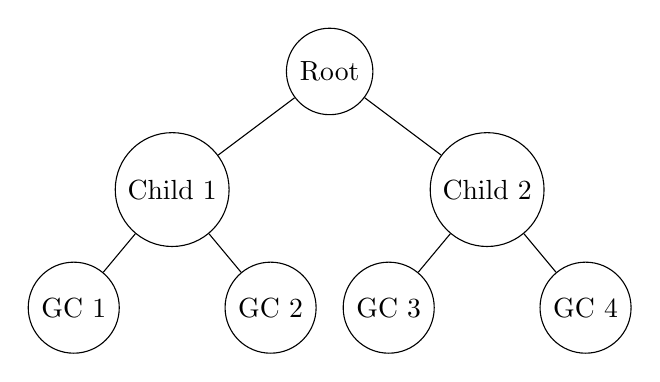
\begin{tikzpicture}[
		level 1/.style={sibling distance=4cm},
		level 2/.style={sibling distance=2.5cm},
		every node/.style={draw, circle, minimum size=1cm}
		]
		
		\node {Root}
		child {node {Child 1}
			child {node {GC 1}}
			child {node {GC 2}}
		}
		child {node {Child 2}
			child {node {GC 3}}
			child {node {GC 4}}
		};
		
	\end{tikzpicture}
	
\end{document}

"""

Lab 11

"""

\documentclass{article}
\usepackage{algorithm}
\usepackage{algorithmic}

\begin{document}
	
	\section{Algorithm using \texttt{algorithm} and \texttt{algorithmic} Packages}
	
	\begin{algorithm}
		\caption{Example Algorithm}\label{alg:example1}
		
		\begin{algorithmic}[1]
			
			\REQUIRE $n \geq 0$
			\ENSURE $y = x^n$
			
			\STATE $y \gets 1$
			\STATE $x \gets x_0$
			\STATE $n \gets n_0$
			
			\WHILE{$n \neq 0$}
			
			\IF{$n$ is even}
			\STATE $x \gets x \times x$
			\STATE $n \gets n / 2$
			\ELSE
			\STATE $y \gets y \times x$
			\STATE $n \gets n - 1$
			\ENDIF
			
			\ENDWHILE
			
		\end{algorithmic}
	\end{algorithm}
	
\end{document}

"""

Lab 12 A

"""

\documentclass{report}
\title{My Simple Report}
\author{Your Name}
\date{\today}
\begin{document}
\maketitle
\tableofcontents
\chapter{Introduction}
This is the introduction of my simple report.
\section{Background}
Here, I'll provide some background information.
\chapter{Methods}
This chapter describes the methods used in my study.
\chapter{Results}
Here are the results of my study.
\chapter{Conclusion}
In conclusion, I'll summarize my findings.
\end{document}

"""

Lab 12 B

"""

\documentclass{article}
\title{My Simple Article}
\author{Your Name}
\date{\today}
\begin{document}
\maketitle
\section{Introduction}
This is the introduction of my simple article.
\subsection{Background}
Here, I'll provide some background information.\section{Methods}
This section describes the methods used in my study.
\section{Results}
Here are the results of my study.
\section{Discussion}
I'll discuss the implications of the results in this section.
\section{Conclusion}
In conclusion, I'll summarize my findings.
\end{document}

"""
